Prácticamente la totalidad de los protocolos de encaminamiento modernos fundamentan sus decisiones en algún criterio de optimización, siendo el de \textbf{mínimo coste} el más extendido. Bajo este paradigma, la red se modela como un grafo donde los nodos representan conmutadores y las aristas representan los enlaces de comunicación, cada uno con un peso o coste asociado.

Dada una red de nodos conectados por enlaces bidireccionales, el coste de una ruta se define como la suma algebraica de los costes de los enlaces individuales que la componen. Es importante destacar que el coste de un enlace puede ser asimétrico (variar según el sentido de la transmisión). La mayoría de los algoritmos utilizados en la actualidad son variantes de dos algoritmos fundamentales de la teoría de grafos: Dijkstra y Bellman-Ford.

\subsection{Algoritmo de Dijkstra}

El algoritmo de Dijkstra, también denominado \textit{Shortest Path First} (SPF), es un algoritmo de tipo \textbf{estado de enlace} (\textit{link-state}). Su objetivo es hallar las rutas de mínimo coste desde un nodo origen específico hacia todos los demás nodos de la red. Para su correcta ejecución, requiere que el nodo origen posea un conocimiento global de la topología de la red.

El procedimiento se desarrolla de forma iterativa, construyendo los caminos en orden creciente de longitud. Se definen los siguientes conceptos clave:

\begin{itemize}
	\item $N$: Conjunto de todos los nodos de la red.
	\item $s$: Nodo origen desde el cual se calculan las rutas.
	\item $T$: Conjunto de nodos para los cuales ya se ha determinado la ruta de mínimo coste (etiquetados permanentemente).
	\item $w(i,j)$: Coste directo del enlace del nodo $i$ al nodo $j$ ($ \infty $ si no existe conexión directa).
	\item $L(n)$: Coste acumulado del camino más corto conocido actualmente desde $s$ hasta $n$.
\end{itemize}

El algoritmo itera siguiendo tres pasos fundamentales hasta que todos los nodos de la red han sido incorporados al conjunto $T$:

\subsubsection{Inicialización}

Se comienza con el nodo origen en el conjunto de rutas conocidas: $T = \{s\}$. Para cada nodo $n \in N$ tal que $n \neq s$, se establece el coste inicial $L(n)$ como el peso del enlace directo desde el origen: $L(n) = w(s,n)$.

\subsubsection{Selección del nodo óptimo}

Se identifica un nodo $x$ que no pertenezca a $T$ y que posea el valor de $L(x)$ más pequeño entre todos los candidatos. Este nodo se incorpora de forma permanente al conjunto $T$, ya que se garantiza que no existe un camino más corto hacia él.

\subsubsection{Actualización de etiquetas}

Para todos los nodos $n \notin T$ que son vecinos de $x$, se evalúa si la ruta actual hacia $n$ puede mejorarse transitando a través de $x$. La actualización se realiza mediante la expresión: 
\[ L(n) = \min[L(n), L(x) + w(x,n)] \]

\subsection{Algoritmo de Bellman-Ford}

El algoritmo de Bellman-Ford constituye la base de los protocolos de \textbf{vector-distancia}. A diferencia de Dijkstra, es un procedimiento intrínsecamente descentralizado; cada nodo solo requiere información de sus vecinos directos para que la red converja globalmente a la solución óptima.

Los conceptos fundamentales utilizados en su formulación iterativa son:

\begin{itemize}
	\item $s$: Nodo origen.
	\item $h$: Índice de iteración, que representa el número máximo de enlaces (saltos) permitidos en la ruta.
	\item $L_h(n)$: Coste del camino mínimo desde $s$ hasta $n$ utilizando como máximo $h$ enlaces.
\end{itemize}

\subsubsection{Inicialización}

En la etapa inicial ($h=0$), el coste hacia el propio origen es nulo ($L_0(s)=0$), mientras que para cualquier otro nodo $n$, el coste se asume infinito ($L_0(n)=\infty$).

\subsubsection{Actualización Iterativa}

En cada etapa sucesiva $h+1$, el algoritmo busca mejorar el coste hacia cada nodo $n$ considerando las rutas que pasan por sus vecinos $j$:
\[ L_{h+1}(n) = \min_j [L_h(j) + w(j,n)] \]

Este proceso de intercambio de vectores de distancia entre vecinos continúa hasta que no se detectan mejoras en los costes (\textit{convergencia}), lo que garantiza que se ha hallado el camino óptimo, siempre que la red no contenga ciclos de coste total negativo.

\begin{figure}[H]
	\centering
	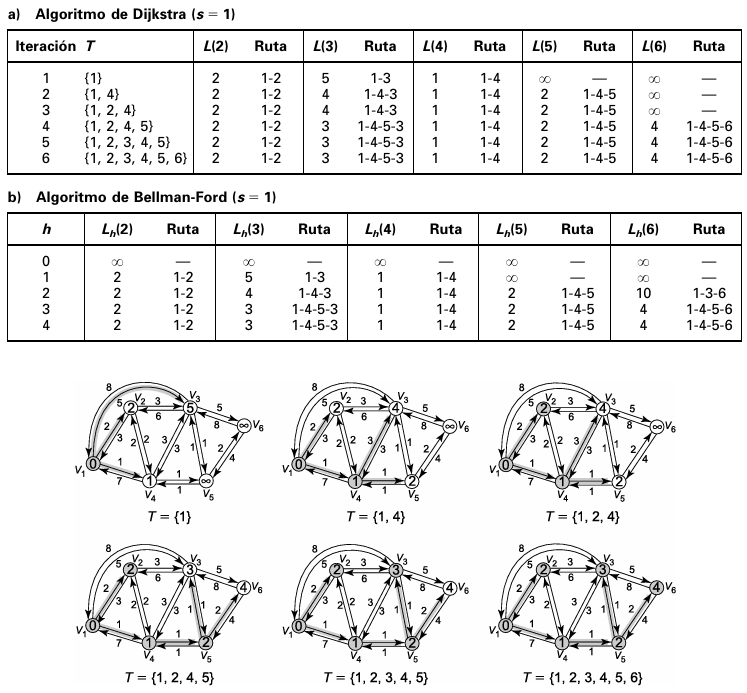
\includegraphics[width=0.9\textwidth]{img/algoritmos.png}
	\caption{Comparativa visual de la ejecución de los algoritmos de Dijkstra y Bellman-Ford.}
	\label{fig:grafico6}
\end{figure}
